\documentclass[tikz,border=12pt]{standalone}
\usepackage[T1]{fontenc}
\usepackage{tgheros}
\usepackage{sfmath}
\usepackage{amsmath}
\usepackage{amssymb}
\usepackage{fontawesome5}
\usepackage{tikz}
\usetikzlibrary{arrows.meta,positioning,shapes.geometric,fit,backgrounds,calc}
\usepackage{xcolor}

\renewcommand{\familydefault}{\sfdefault}

% Harvard Crimson & ETH Zurich Academic Semantic Palette
\definecolor{harvardcrimson}{HTML}{A51C30}
\definecolor{ethdarkblue}{HTML}{1F407A}
\definecolor{ethblue}{HTML}{215CAF}
\definecolor{ethpetrol}{HTML}{007A87}
\definecolor{ethbronze}{HTML}{B87333}
\definecolor{ethpurple}{HTML}{5B4B8A}
\definecolor{ethslate}{HTML}{475569}
\definecolor{cardbg}{HTML}{F8FAFC}
\definecolor{cardborder}{HTML}{CBD5E1}
\definecolor{safeTeal}{HTML}{10B981}
\definecolor{alertRed}{HTML}{DC2626}

\begin{document}
\begin{tikzpicture}[
  font=\sffamily,
  >=Stealth
]

  % Top Title Banner
  \node[draw=ethdarkblue, fill=ethdarkblue!5, rounded corners=5pt, line width=1pt, text width=9.00in, inner sep=7pt, align=center] (title) at (4.50in, 0) {
    {\normalsize\bfseries\color{ethdarkblue}\faIcon{stopwatch}\;\; MULTI-SENSOR HARDWARE SYNCHRONIZATION \& TIMESTAMP METROLOGY}\\[2pt]
    {\scriptsize\color{ethslate}Eliminating the Software Timestamp Illusion via PTP Hardware Strobes and Exposure Integration Midpoints}
  };

  % Timeline Axis
  \draw[->, line width=1.1pt, draw=ethdarkblue] (0, -0.65in) -- (9.00in, -0.65in)
    node[right, font=\scriptsize\bfseries, text=ethdarkblue] {Time $t$};

  % Time ticks
  \foreach \x/\txt in {1.0/0\text{ ms}, 3.0/10\text{ ms}, 5.0/20\text{ ms}, 7.0/30\text{ ms}, 8.5/40\text{ ms}} {
    \draw[line width=0.6pt, draw=ethslate!50] (\x in, -0.60in) -- (\x in, -0.70in)
      node[below, font=\tiny\color{ethslate}] {\txt};
  }

  % Row 1: Camera Exposure & Readout
  \node[anchor=west, font=\scriptsize\bfseries\color{ethblue}] at (0, -1.15in) {\faIcon{camera}\; Camera (30 Hz RGB-D):};

  % Exposure block
  \draw[fill=ethblue!20, draw=ethblue, line width=0.9pt, rounded corners=2pt] (1.0in, -1.45in) rectangle ++(1.6in, 0.40in);
  \node[font=\tiny\bfseries\color{ethblue}] at (1.8in, -1.25in) {Exposure ($t_{\text{exp}} = 8\text{ ms}$)};

  % Readout DMA block
  \draw[fill=ethslate!20, draw=ethslate, line width=0.8pt, rounded corners=2pt] (2.6in, -1.45in) rectangle ++(1.4in, 0.40in);
  \node[font=\tiny\bfseries\color{ethslate}] at (3.3in, -1.25in) {MIPI DMA ($7\text{ ms}$)};

  % True Physical Midpoint vs Software Arrival
  \draw[dashed, line width=1pt, draw=safeTeal] (1.8in, -0.65in) -- (1.8in, -1.85in);
  \node[font=\tiny\bfseries, fill=white, draw=safeTeal, rounded corners=2pt, inner sep=2pt, text=safeTeal] at (1.8in, -1.95in) {
    \faIcon{check}\; True Hardware Midpoint ($t_{\text{mid}} = T+4\text{ ms}$) [PTP Strobe]
  };

  \draw[dashed, line width=1pt, draw=alertRed] (4.0in, -0.65in) -- (4.0in, -1.85in);
  \node[font=\tiny\bfseries, fill=white, draw=alertRed, rounded corners=2pt, inner sep=2pt, text=alertRed] at (4.0in, -2.15in) {
    \faIcon{times}\; Naive Software Timestamp ($t_{\text{sw}} = T+15\text{ ms}$) [Late by $11\text{ ms}$!]
  };

  % Row 2: IMU High-Rate Samples
  \node[anchor=west, font=\scriptsize\bfseries\color{ethpetrol}] at (0, -2.60in) {\faIcon{tachometer-alt}\; IMU (1000 Hz SPI):};
  \foreach \i in {1.0, 1.4, 1.8, 2.2, 2.6, 3.0, 3.4, 3.8, 4.2, 4.6, 5.0, 5.4, 5.8, 6.2, 6.6, 7.0, 7.4, 7.8, 8.2} {
    \draw[line width=1pt, draw=ethpetrol] (\i in, -2.50in) -- (\i in, -2.75in);
    \draw[fill=ethpetrol] (\i in, -2.75in) circle (1.2pt);
  }
  \node[anchor=west, font=\tiny\color{ethpetrol}] at (8.3in, -2.62in) {$\Delta t = 1.0\text{ ms}$};

  % Bottom Section: Comparison of Alignment
  \node[draw=cardborder, fill=cardbg, rounded corners=4pt, line width=0.8pt, text width=8.80in, inner sep=6pt, align=left] (footer) at (4.50in, -3.45in) {
    {\scriptsize\bfseries\color{ethdarkblue}\faIcon{info-circle}\; CRITICAL SYNCHRONIZATION LAWS IN PHYSICAL PERCEPTION:}\\[3pt]
    {\tiny\color{ethslate}
    $\bullet$ \textbf{Motion Blur Uncertainty:} Moving at velocity $v = 1.5\text{ m/s}$ with $t_{\text{exp}} = 10\text{ ms}$ blurs visual features across $\Delta x = v \cdot t_{\text{exp}} = \mathbf{15\text{ mm}}$ of spatial smear.\\
    $\bullet$ \textbf{Temporal Skew Illusion:} Correlating an image with an IMU reading using software timestamps creates an $11\text{ ms}$ phase mismatch, inducing catastrophic drift in Kalman state estimators.\\
    $\bullet$ \textbf{PTP (IEEE 1588) Solution:} The image sensor triggers a hardware GPIO strobe at exposure start. The PTP timer registers the true physical midpoint ($t_{\text{mid}} = t_{\text{start}} + \frac{1}{2}t_{\text{exp}}$) with sub-microsecond precision.
    }
  };

\end{tikzpicture}
\end{document}
